%% Submissions for peer-review must enable line-numbering
%% using the lineno option in the \documentclass command.
%%
%% Preprints and camera-ready submissions do not need
%% line numbers, and should have this option removed.
%%
%% Please note that the line numbering option requires
%% version 1.1 or newer of the wlpeerj.cls file, and
%% the corresponding author info requires v1.2

\documentclass[fleqn,10pt]{wlpeerj} % for preprint submissions

% ZNK -- Adding headers for pandoc

\setlength{\emergencystretch}{3em}
\providecommand{\tightlist}{
\setlength{\itemsep}{0pt}\setlength{\parskip}{0pt}}
\usepackage{lipsum}
\usepackage[unicode=true]{hyperref}
\usepackage{longtable}



\usepackage{lipsum} \usepackage{multirow}

\title{Juvenile Salmon Migration Dynamics in the Discovery Islands and
Johnstone Strait in 2018}

\author[1]{Brett T. Johnson}

\corrauthor[1]{Brett T. Johnson}{\href{mailto:brett.johnson@hakai.org}{\nolinkurl{brett.johnson@hakai.org}}}
\author[]{Julian C.L. Gan}

\author[]{Carly V. Janusson}

\author[2, 3]{Brian P.V. Hunt}


\affil[1]{Hakai Institute Quadra Island Ecological Observatory, Heriot Bay, BC
V0P1H0}
\affil[2]{UBC EOS, IOF}


%
% \author[1]{First Author}
% \author[2]{Second Author}
% \affil[1]{Address of first author}
% \affil[2]{Address of second author}
% \corrauthor[1]{First Author}{f.author@email.com}

% 

\begin{abstract}
The majority of out-migrating juvenile Fraser River salmon
(\emph{Oncorhynchus} spp.) pass northwest through the Strait of Georgia,
the Discovery Islands, and Johnstone Strait. The Discovery Islands to
Johnstone Strait leg of the migration is a region of poor survival for
juvenile salmon relative to the Strait of Georgia. The Hakai Institute
Juvenile Salmon Program has been monitoring key components of this
migration since 2015 to better understand drivers of early marine
survival. Here we present key aspects of the 2018 migration in
comparison to averages from the 2015--2018 study period, which we use to
define `normal'. In 2018 sockeye (\emph{Oncorhynchus nerka}), pink
(\emph{O. gorbuscha}), and chum (\emph{O. keta}) all migrated earlier
than normal. The median capture date was May 23rd for sockeye, five days
earlier than normal; and June 12 for pink and chum, which is five days
earlier for pink and three days earlier than normal for chum. Sea lice
prevalence was lower than normal for sockeye, pink, and chum. Notably,
there were no \emph{Lepeophtheirus salmonis} sea lice observed in
Johnstone Strait in 2018. Sockeye were longer than normal in 2018
whereas pink and chum were smaller than normal. Sea surface temperatures
in May and June were the warmest on record in the study period
(2015--2018). Pink salmon dominated the catch in 2018, followed by chum,
and then sockeye.
% Dummy abstract text. Dummy abstract text. Dummy abstract text. Dummy abstract text. Dummy abstract text. Dummy abstract text. Dummy abstract text. Dummy abstract text. Dummy abstract text. Dummy abstract text. Dummy abstract text.
\end{abstract}

\begin{document}

\flushbottom
\maketitle
\thispagestyle{empty}

\section*{Introduction}\label{introduction}
\addcontentsline{toc}{section}{Introduction}

Pacific salmon (\emph{Oncorhynchus} spp.) traverse a number of aquatic
landscapes during different phases of their lifecycle. During their
migrations, salmon are subjected to risks associated with each new
environment they encounter. The risks and associated mortality from the
sum of these migrations can be understood in aggregate by quantifying
the productivity (recruits per spawner) of a certain stock. Salmon are
an excellent indicator species because they integrate terrestrial,
lacustrine, fluvial, estuarine, nearshore marine, and high-seas
conditions; a problem in any one of these environments will be reflected
in the productivity of salmon stocks. To better manage and predict the
productivity of salmon stocks we need estimates of mortality and an
understanding of the factors driving mortality in each landscape that
salmon traverse. One such area in which we lack understanding is the
early marine environment. Juvenile salmon are particularly vulnerable
during the early marine phase of their life history because they are
undergoing physiological adaptations to a saline environment.

The Hakai Institute Juvenile Salmon Program has been monitoring juvenile
salmon migrations in the Discovery Islands and Johnstone Strait (Figure
\ref{fig:map}) since 2015 in an effort to understand what factors may be
influencing early marine survival of sockeye, pink, and chum (Hunt et
al. 2018). The effects of pathogens, parasites, predators, and the
impacts of climate change on food web dynamics may be amplified during
this stressful transition period. Factors on which we are currently
monitoring and reporting include migration dynamics, growth, parasites
and pathogens, and the ocean's physical condition.

\begin{figure}

\includegraphics[width=0.8\linewidth]{map} \hfill{}

\caption{Sampling locations in 2018}\label{fig:map}
\end{figure}

\section*{Methods}\label{methods}
\addcontentsline{toc}{section}{Methods}

\subsection*{Field methods}\label{field-methods}
\addcontentsline{toc}{subsection}{Field methods}

See Hunt et al. (2018) for a detailed description of field and lab
methods. Briefly, we collect juvenile salmon weekly from the Discovery
Islands and Johnstone Strait during their northward migration from the
Strait of Georgia to Queen Charlotte Strait near northern Vancouver
Island, British Columbia. Sampling is conducted from May to July each
year since 2015 using purse seine nets (bunt: 27 m x 9 m with 13 mm
mesh; tow: 46 m x 9 m with 76 mm mesh). We sample in nearshore marine
habitats with depth \textgreater{} 10 m and effectively sample sockeye
(\emph{Oncorhynchus nerka}), pink (\emph{O. gorbuscha}), chum (\emph{O.
keta}) and incidentally capture coho (\emph{O. kisutch}), chinook
(\emph{O. tshawytschya}) and Pacific herring (\emph{Clupea pallasii}).
All animal care was in accordance with Animal Care Guidelines under
permit A16-0101. Temperature data were collected by deploying an RBR
conductivity, temperature, and depth profiler to depths \textgreater{}
30 m at station QU39 ( Figure \ref{fig:map}) in the northern Strait of
Georgia.

\subsection*{Statistical methods}\label{statistical-methods}
\addcontentsline{toc}{subsection}{Statistical methods}

All metrics reported are in relation to the time series average
(2015-2018). The mean for each parameter of interest was calculated for
all years combined, and the z-score was calculated for each parameter to
determine the number of standard deviations away from the mean a given
parameter was in each year.

\(Z = {\frac{x_i - \bar X}{{S}}}\)

Annual migration timing for each species was measured by calculating the
median date of capture in the Discovery Islands, the date at which the
50 percent of the fish passed through the region. To visualize migration
timing we plotted cumulative catch abundance between May 1st and July
9th each year and fit a logistic growth line. Species proportions were
calculated by dividing the total number of each species caught that
season across all seines by the sum of all species caught that season.
Fork length distributions were visualized by calculating density
estimates from fork length data. The prevalence of sealice was
calculated as the number of individuals of a host species infected with
a particular parasite species divided by Number of hosts examined
(Margolis et al. 1990). Sea surface was defined as the top 30 m of the
water column. The mean temperature from which to compare any single year
to was calculated from the top 30 m of the water column in May and June
from all years. To visualize temperature anomalies we applied a loess
regression to sea surface temperatures from all four years to develop a
model that would represent the seasonal trend.

\section*{Results}\label{results}
\addcontentsline{toc}{section}{Results}

The heatmap below summarizes the amount of variation each parameter
exhibits over the past four years by visualizing the number of standard
deviations from the time-series average (Z-score) (Figure
\ref{fig:heatmap}). Peak migration date, parasite loads, and fork
lengths were all calculated for sockeye.

Sea-surface temperatures in May and June at QU39 were warmer than
normal, or 1.33 standard deviations greater than the time series mean.
The peak migration date in the Discovery Islands occurred earlier than
average in 2018 (-0.71 SD). Across the Discovery Islands and Johnstone
Strait, parasite loads were lower than average (-0.98 SD), and fork
lengths were longer than average (0.62 SD).

\begin{figure}
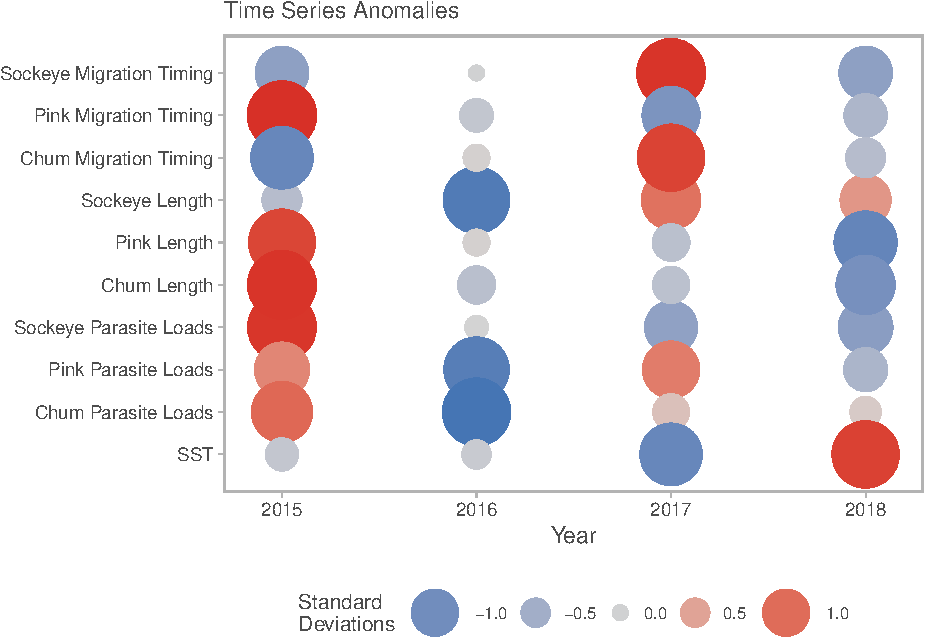
\includegraphics[width=0.8\linewidth]{peer_j_migration_dynamics_files/figure-latex/heatmap-1} \caption{This heatmap indicates the number of standard deviations (Z-score) from the time series average (2015-2018) for key migration parameters. Blue colour indicates less than average, white indicates average, red indicates greater than average. Peak migration date is based on the median date of sockeye capture in the Discovery Islands.  Mean sea-surface temperature is 30 m depth integrated temperature from station QU39 in the Northern Strait of Georgia from May and June. Parasite load is the average prevalence of all sea lice species in their motile life stage for both the Discovery Islands and Johnstone Strait regions combined.}\label{fig:heatmap}
\end{figure}

\subsection*{Migration Timing}\label{migration-timing}
\addcontentsline{toc}{subsection}{Migration Timing}

The bulk of the sockeye migration in the Discovery Islands occurred
earlier in 2018 when compared to the time-series's four-year average
(Figure \ref{fig:mt}). The median date of capture for 2018 sockeye was
May 22nd, whereas the time series average was May 27th. Conversely, the
2018 sockeye migration occurred later than normal in Johnstone Strait,
where the median date of capture was June 6th, which is two days later
than the time-series average. See Table @ref(tab:mt\_di) and Table
@ref(tab:mt\_js) for the interqurtile range of migration timing for
sockeye, pink, and chum in 2018, contrasted to the time series averages
for the Discovery Islands and Johnstone Strait, respectively. Based on
the comparison of peak migration dates between the two zones, we
estimate that the average residence time of juvenile salmon in the
Discovery Islands for 2018 was approximately two weeks.

\begin{figure}
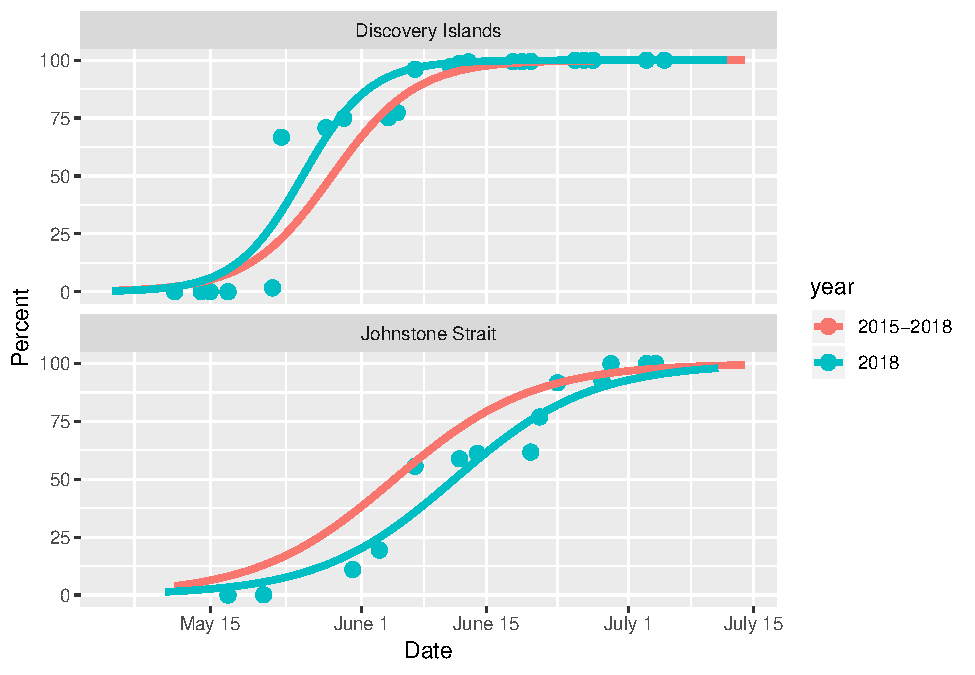
\includegraphics[width=0.8\linewidth]{peer_j_migration_dynamics_files/figure-latex/mt-1} \caption{Cumulative catch of juvenile sockeye salmon migrating through the Discovery Islands compared to the average for 2015--2018. Migration curves were predicted by fitting a logistic growth equation to the cumulative percent the selected fish caught. The points (circles) for the year being compared to the time-series is the cumulative catch percent}\label{fig:mt}
\end{figure}

\begin{table}[ht]
\centering
\begin{tabular}{l|l||c|c|c}
\multicolumn{5}{c}{\textbf{Discovery Islands}} \\
\hline
\textbf{Species} & \textbf{Year} & \textbf{25\%} & \textbf{50\%} & \textbf{75\%} \\
\hline
\multirow{2}{*}{Sockeye} & TSA & May 25 & May 27 & June 03 \\
& 2018 & May 22 & May 22 & June 03 \\
\hline
\multirow{2}{*}{Pink} & TSA & June 04 & June 12 & June 15 \\
& 2018 & June 06 & June 11 & June 17 \\
\hline
\multirow{2}{*}{Chum} & TSA & June 05 & June 14 & June 21 \\
& 2018 & June 06 & June 11 & June 19 \\
\end{tabular}
\caption{\label{tab:mt_di}Interquartile range for the cumulative catch of sockeye, pink, and chum salmon in the Discovery Islands in 2018, compared to the Time-Series Average (2015--2018). Odd years were excluded from the TSA calculation for pink salmon due being the "off" years in the outmigration cycle.}
\end{table}

\begin{table}[ht]
\centering
\begin{tabular}{l|l||c|c|c}
\multicolumn{5}{c}{\textbf{Johnstone Strait}} \\
\hline
\textbf{Species} & \textbf{Year} & \textbf{25\%} & \textbf{50\%} & \textbf{75\%} \\
\hline
\multirow{2}{*}{Sockeye} & TSA & June 01 & June 04 & June 17 \\
& 2018 & June 06 & June 06 & June 20 \\
\hline
\multirow{2}{*}{Pink} & TSA & June 15 & June 21 & June 22 \\
& 2018 & June 13 & June 20 & June 22 \\
\hline
\multirow{2}{*}{Chum} & TSA & June 10 & June 17 & June 25 \\
& 2018 & June 13 & June 20 & June 27 \\
\end{tabular}
\caption{\label{tab:mt_js}Interquartile range for the cumulative catch of sockeye, pink, and chum salmon in Johnstone Strait in 2018, compared to the Time-Series Average (2015--2018). Odd years were excluded from the TSA calculation for pink salmon due being the "off" years in the outmigration cycle.}
\end{table}

\subsection*{Species Proportions}\label{species-proportions}
\addcontentsline{toc}{subsection}{Species Proportions}

Pink salmon dominated the catch in the Discovery Islands and Johnstone
Strait in 2018, which is the first time observed in the time-series
(Figure \ref{fig:prop}). This may be due to post-smolts being from the
dominant odd-year pink returning broodlines (Krkošek et al. 2011;
Beacham et al. 2012; Irvine et al. 2014) coupled with Fraser River
sockeye from the weak 2016 brood year, which was lowest recorded return
in 100 years (McKinnell et al. 2012; Grant, MacDonald, and Michielsens
2017; Pacific Salmon Commission 2017).

\begin{figure}
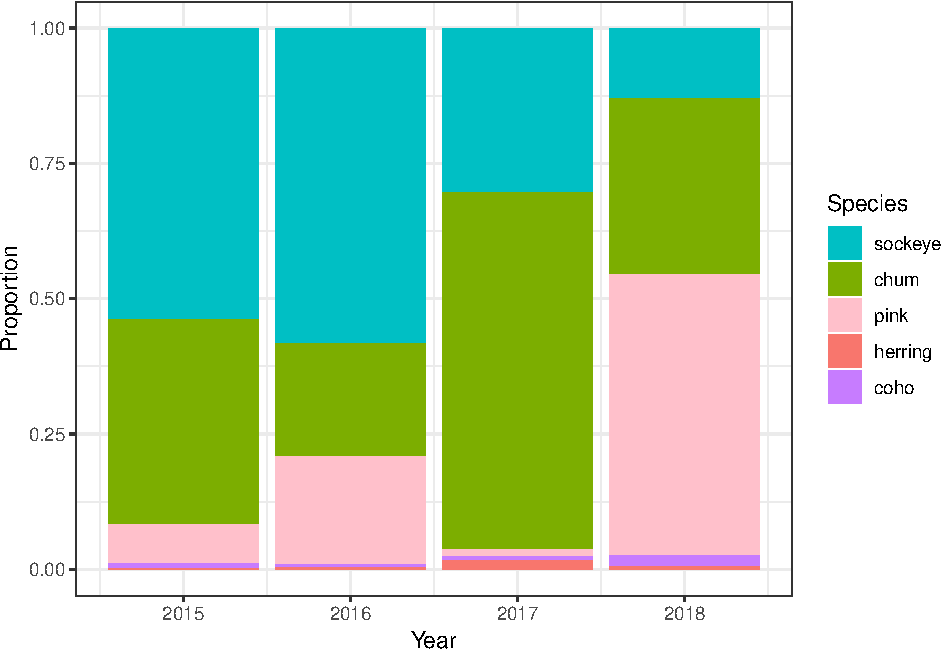
\includegraphics[width=0.8\linewidth]{peer_j_migration_dynamics_files/figure-latex/prop-1} \caption{The annual proportion of fish captured in the Discovery Islands and Johnstone Strait combined.}\label{fig:prop}
\end{figure}

\subsection*{Length}\label{length}
\addcontentsline{toc}{subsection}{Length}

Fish lengths varied between regions, species and year (Figure
\ref{fig:length}). Sockeye were longer than average in 2018\ldots{}

\begin{figure}
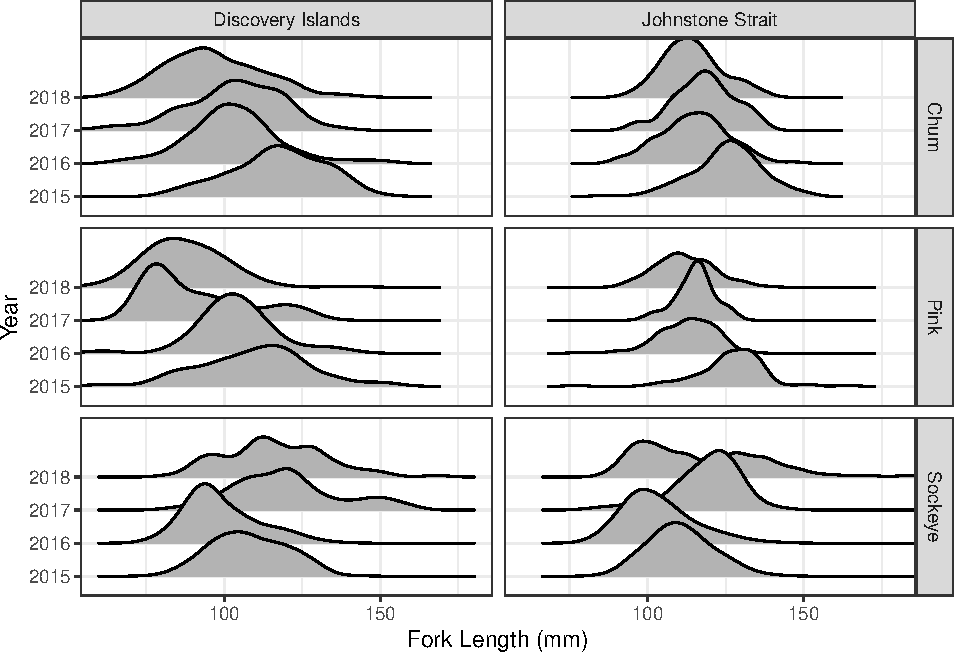
\includegraphics[width=0.8\linewidth]{peer_j_migration_dynamics_files/figure-latex/length-1} \caption{Kernel density distributions of juvenile salmon fork lengths for each year in the selected region. Note that these distributions contain multiple age-classes.}\label{fig:length}
\end{figure}

\subsection*{Parasite Loads}\label{parasite-loads}
\addcontentsline{toc}{subsection}{Parasite Loads}

The prevalence of motile (pre-adult and adult life stage) sea lice in
2018 was the lowest recorded in the time-series (Figure
\ref{fig:sealice}). Notably, no \emph{Lepeophtheirus salmonis} were
detected on sockeye in Johnstone Strait, despite being present in the
Discovery Islands. Pink salmon appeared to have higher counts of
\emph{Caligus clemensi} in 2018 compared to chum and sockeye.

\begin{figure}
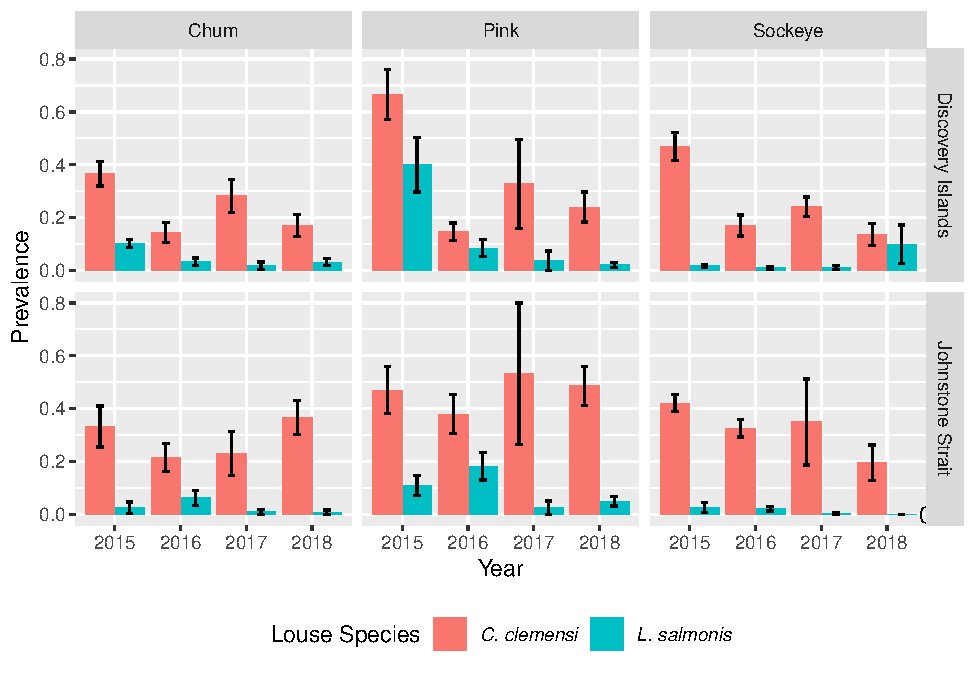
\includegraphics[width=0.8\linewidth]{peer_j_migration_dynamics_files/figure-latex/sealice-1} \caption{The prevalence (+/-SE) of motile sea lice on juvenile salmon in the Discovery Islands and Johnstone Strait.}\label{fig:sealice}
\end{figure}

\subsection*{Sea Surface Temperature}\label{sea-surface-temperature}
\addcontentsline{toc}{subsection}{Sea Surface Temperature}

Sea surface temperature was warm (Figure \ref{fig:sst})

\begin{figure}
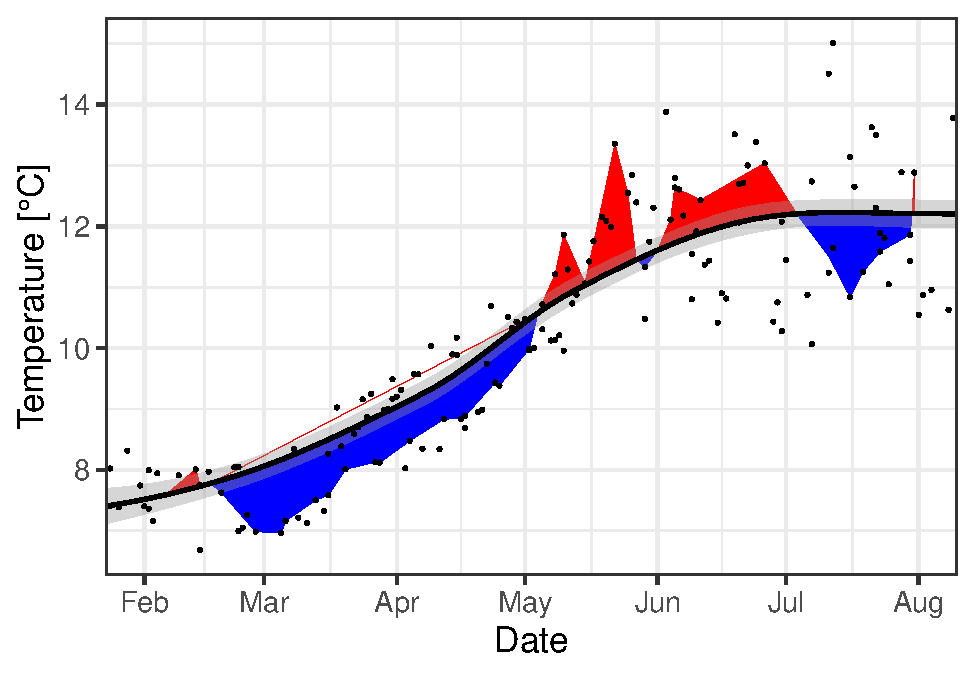
\includegraphics[width=0.8\linewidth]{peer_j_migration_dynamics_files/figure-latex/sst-1} \caption{Time series of 30 m depth integrated temperature anomalies observed at Hakai Oceanographic Monitoring station QU39. Blue areas represent temperatures that are below normal, red areas represent above normal temperatures at the selected station in 2018. Normal is the solid black line which is a loess regression based on temperatures from 2015-2018. The shaded grey area is 1 SE of the loess regression. The black dots are the daily minimum and maximum temperatures observed over the time series.}\label{fig:sst}
\end{figure}

\section*{Discussion}\label{discussion}
\addcontentsline{toc}{section}{Discussion}

\hypertarget{refs}{}
\hypertarget{ref-Beacham2012}{}
Beacham, Terry D., Brenda Mcintosh, Cathy MacConnachie, Brian Spilsted,
and Bruce A. White. 2012. ``Population structure of pink salmon
(Oncorhynchus gorbuscha) in British Columbia and Washington, determined
with microsatellites.'' \emph{Fishery Bulletin} 110 (2): 242--56.
doi:\href{https://doi.org/10.2337/diabetes.51.4.1093}{10.2337/diabetes.51.4.1093}.

\hypertarget{ref-Grant2017}{}
Grant, S C H, Bronwyn L MacDonald, and Catherine GJ Michielsens. 2017.
``Fraser River Sockeye: Abundance and Productivity Trends and
Forecasts.'' North Pacific Anadromous Fish Commission.
\url{http://www.npafc.org}.

\hypertarget{ref-Irvine2014}{}
Irvine, J R, C. J.G. Michielsens, M. O'Brien, B A White, and M Folkes.
2014. ``Increasing Dominance of Odd-Year Returning Pink Salmon.''
\emph{Transactions of the American Fisheries Society} 143 (4): 939--56.
doi:\href{https://doi.org/10.1080/00028487.2014.889747}{10.1080/00028487.2014.889747}.

\hypertarget{ref-Krkosek2011}{}
Krkošek, Martin, Ray Hilborn, Randall M. Peterman, and Thomas P. Quinn.
2011. ``Cycles, stochasticity and density dependence in pink salmon
population dynamics.'' \emph{Proceedings of the Royal Society B:
Biological Sciences} 278 (1714). The Royal Society: 2060--8.
doi:\href{https://doi.org/10.1098/rspb.2010.2335}{10.1098/rspb.2010.2335}.

\hypertarget{ref-Margolis1990}{}
Margolis, L., G. W. Esch, A.M. Kuris, and G.A. Schad. 1990. ``The Use of
Ecological Terms in Parasitology (Report of an Ad Hoc Committee of the
American Society of Parasitologists).'' \emph{The Journal of
Parisitology} 68 (1): 131--33.
doi:\href{https://doi.org/10.2307/3281335}{10.2307/3281335}.

\hypertarget{ref-McKinnell2012}{}
McKinnell, S.M., E. Curchitser, C. Groot, M. Kaeriyama, and K.W. Myers.
2012. ``PICES Advisory Report on the decline of Fraser River Sockeye
Salmon Oncorhynchus nerka (Steller, 1743) in relation to marine
ecology.'' \emph{PICES Sci. Rep.} No. 41 (February): 149 pp.

\hypertarget{ref-PacificSalmonCommission2017}{}
Pacific Salmon Commission. 2017. ``Report of the Fraser River Panel to
the Pacific Salmon Commission on the 2016 Fraser River Sockeye Salmon
Fishing Season.'' Pacific Salmon Commission.
\url{https://www.psc.org/publications/annual-reports/fraser-river-panel/}.



\end{document}
